\clearpage
\section{Altar and Vessel Linens}
Five white linens serve the altar and sacred vessels. Because the corporal and purificator come into direct contact with the Sacred Species, the Church distinguishes them sharply from practical service towels both in fold geometry and in sacristy laundering, requiring first-rinse water to be poured into the sacrarium or clean earth (Redemptionis Sacramentum 120).

\PCDPlateHeader{Plate IV --- Altar and Vessel Linens}{Not to common scale}
\ifdefined\TriptychPrintEdition
\begin{center}
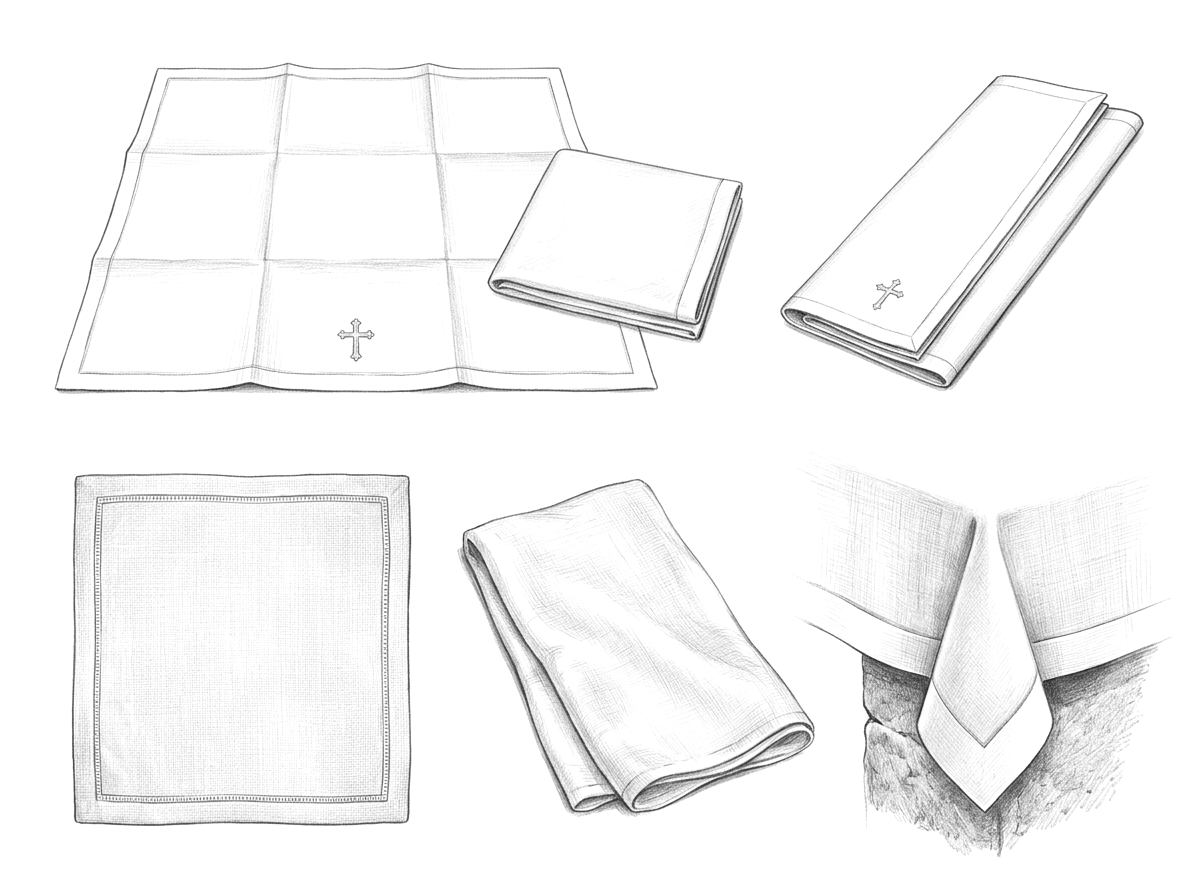
\includegraphics[width=0.92\linewidth,height=3.55in,keepaspectratio]{liturgy/roman-rite/postconciliar/2008-latin-2011-us-english/reference/roman-sanctuary-dictionary/shared/artwork/graphite/pc-art-04-white-linens.png}
\end{center}
\PCDPositionKey{Top left: unfolded square Corporal showing its three-by-three fold grid and front stitched cross, paired with a folded Corporal; top right: oblong Purificator folded lengthwise in thirds with stitched cross visible near the lower folded end; bottom left: stiffened square Pall; bottom center: folded Lavabo Towel; bottom right: hemmed corner of white Altar Cloth draped over the mensa.}
\else
\textbf{Visual Plate Summary (Plate IV --- Altar and Vessel Linens, Not to common scale):} Five-subject monochrome graphite textile study on pure white stock differentiating white altar linens by crease geometry and drape: top left, an unfolded square corporal creased into nine squares with a small stitched cross near the front center edge beside a folded square corporal; top right, an oblong purificator folded lengthwise in thirds with a small stitched cross visible near the lower folded end; bottom left, a rigid flat square linen pall; bottom center, a softly folded rectangular lavabo finger towel; bottom right, a hemmed corner of a white altar cloth hanging over a stone altar edge.

\textbf{Reading order and object placement:} Top left: unfolded square Corporal showing its three-by-three fold grid and front stitched cross, paired with a folded Corporal; top right: oblong Purificator folded lengthwise in thirds with stitched cross visible near the lower folded end; bottom left: stiffened square Pall; bottom center: folded Lavabo Towel; bottom right: hemmed corner of white Altar Cloth draped over the mensa.
\fi

\label{pc-obj-altar-cloth}
\PCDEntryHead{Altar Cloth}{Mappa}{required}{N15}
\PCDField{Also called}{Fair linen; Altar linen; \textit{Mappa altaris}; \textit{Mappae}; \textit{Tobalea}}
A clean white linen cloth dressing the top surface of the altar for every celebration of Mass. At bottom right of Plate IV, a finely hemmed corner of smooth white linen drapes cleanly over the stone edge of the mensa; Plates I and II show it dressing the entire freestanding altar. Proportioned to the altar's shape and size, it may bear restrained hemstitching, woven bands, or subtle lace suited to noble simplicity.

\PCDField{Plate position and status}{Bottom right corner drape (Plate IV); dressing the altar (Plates I--II) (Universal Roman law)}
\PCDField{Placement and liturgical use}{Laid smoothly over the altar mensa before Mass so that at least one clean white cloth always covers the table of sacrifice (GIRM 117, 304). Any under-cloths---including festive colored under-cloths permitted in United States dioceses---lie neatly beneath the white uppermost cloth. Until the Preparation of the Gifts, the dressed mensa remains uncluttered, holding no cruets, stands, or loose papers (GIRM 306).}
\PCDField{United States norm}{In the Dioceses of the United States of America, the confirmed territorial adaptation at GIRM 304 permits additional altar cloths beneath or alongside the primary cloth to bear other colors of Christian honorific or festive significance, provided the uppermost cloth covering the mensa is always white.}
\PCDField{Ministers and server boundary}{Ordinary ministers: Bishop, Priest, Deacon. Server prepares or sets in place before or during Mass: Servers may assist the sacristan in laying or smoothing a clean altar cloth before Mass with clean hands, keeping wax, ink, and unauthorized items off the mensa and reporting any spill of the Precious Blood immediately to the priest or deacon.}
\PCDSafety{Never blot or wash a spill of the Precious Blood on the altar cloth yourself; notify the priest or deacon at once so the spot is washed with water and the ablution poured into the sacrarium (GIRM 280; RS 120). Guard the linen against candle flames and molten wax.}
\PCDField{Distinguish from}{Corporal, Lavabo Towel}
\PCDField{Symbolism}{The white altar cloth expresses reverence for the celebration of the Lord's memorial and the sacred banquet in which his Body and Blood are offered. In the scholastic tradition of St. Thomas Aquinas, the clean linen dressing the altar also evokes the burial cloth of Christ---``And Joseph taking the body wrapped it up in a clean linen cloth'' (Matt 27:59)---calling to mind purity of conscience and the Passion of the Lord. (GIRM 304; St. Thomas Aquinas, Summa Theologiae III, q. 83, a. 3, ad 7; Matt 27:59)}
\PCDField{1962 Roman Missal counterpart}{\PCDTag{materially changed} The 1962 Roman Missal required three clean blessed white linen cloths covering the altar, with the uppermost cloth reaching the ground at both sides (RG 526). Postconciliar law requires at least one white cloth suited to the altar's shape and size (GIRM 117, 304), while the United States adaptation permits additional festive colored under-cloths beneath the white top cloth.}
\PCDEntryRule

\label{pc-obj-corporal}
\PCDEntryHead{Corporal}{Corporale}{required}{N16}
\PCDField{Also called}{Altar corporal; \textit{Palla corporalis}}
A square white linen cloth unfolded at the center of the altar during the Preparation of the Gifts so that every vessel holding the Body and Blood of Christ rests upon it and any sacred fragment is safely gathered. At top left of Plate IV, the corporal appears both unfolded in a crisp three-by-three crease grid of nine equal squares and folded flat beside it; Plate X shows it spread beneath the principal chalice, paten, veiled ciborium, and Communion cups. Woven of fine white linen with a hemmed edge, it ordinarily bears a small stitched cross near the front center border facing the celebrant.

\PCDField{Plate position and status}{Top left, shown unfolded in a 3x3 crease grid and folded beside it (Plate IV); beneath vessels (Plate X) (Universal Roman law)}
\PCDField{Placement and liturgical use}{Prepared neatly folded on the credence table (GIRM 118c), brought to the altar at the Preparation of the Gifts, and spread open at the center of the mensa by the deacon, instituted acolyte, or priest (GIRM 139, 178, 190). After Communion and vessel purification, the minister folds the sides carefully inward---enclosing the upper surface inside---so no microscopic particle of the Sacred Host can scatter (GIRM 183, 192). Unpurified vessels left on the altar or credence table after Mass likewise rest suitably covered on a corporal (GIRM 279).}
\PCDField{United States norm}{Universal Roman law requires a corporal beneath all Eucharistic vessels on the altar (GIRM 118c, 139, 306) and beneath unpurified vessels awaiting post-Mass purification (GIRM 279; USCCB Norms for Holy Communion under Both Kinds 53). While GIRM 118c commends the optional chalice veil, it does not mention the stiff burse, which remains purely a traditional accessory.}
\PCDField{Ministers and server boundary}{Ordinary ministers: Bishop, Priest, Deacon, Instituted acolyte. Server prepares or sets in place before or during Mass: Servers may set a clean, folded corporal on the credence table before Mass and bring it to the altar at the Preparation of the Gifts when no deacon or instituted acolyte serves; after consecration, servers never shake, refold carelessly, or wash a used corporal, and move a folded corporal flat and level only when directed after purification.}
\PCDSafety{A used corporal may hold fine particles of the Sacred Host. Never shake it out or wash it directly in an ordinary sink; first soak and hand-rinse it in a dedicated basin and pour that first rinse water into the sacrarium or directly into clean earth before ordinary laundering (RS 120).}
\PCDField{Distinguish from}{Purificator, Pall, Lavabo Towel, Altar Cloth}
\PCDField{Symbolism}{Named from the Latin corpus (``body''), the corporal is made of pure white linen because Christ's body was wrapped in a clean linen shroud at his burial: ``And Joseph taking the body wrapped it up in a clean linen cloth'' (Matt 27:59; cf. John 20:6, ``and saw the linen cloths lying''). Following ancient Roman tradition expounded by St. Thomas Aquinas, the white linen signifies purity of conscience and recalls the Passion of Christ. (St. Thomas Aquinas, Summa Theologiae III, q. 83, a. 3, ad 7 (citing De Consecr. dist. 1); Matt 27:59; John 20:6)}
\PCDField{1962 Roman Missal counterpart}{\PCDTag{continued} The square white linen corporal folded inward in nine squares continues directly from the 1962 Roman Missal (RS I.1). In postconciliar Mass with a congregation, it is placed on the altar at the Preparation of the Gifts rather than drawn from a stiff burse at the start of Low Mass (1962 RS II.2), and GIRM 118c no longer mandates a burse.}
\PCDEntryRule

\label{pc-obj-purificator}
\PCDEntryHead{Purificator}{Purificatorium}{required}{N17}
\PCDField{Also called}{Chalice cloth}
An oblong white absorbent linen cloth used to wipe the rim of the chalice during Communion and to dry the chalice, paten, and ciboria after purification. At top right of Plate IV, the oblong linen cloth is folded lengthwise into thirds with a small stitched cross visible on the folded face; Plate X shows a folded purificator paired beside each footed Communion cup. Its narrow triple-folded form and small cross distinguish it clearly from both the square nine-fold corporal and the plain, uncrossed lavabo towel.

\PCDField{Plate position and status}{Top right, folded lengthwise in thirds with stitched cross visible near the lower folded end (Plate IV); beside Communion cups (Plate X) (Universal Roman law)}
\PCDField{Placement and liturgical use}{Prepared on the credence table draped across the principal chalice---and paired one-to-one beside every additional Communion chalice whenever Communion is distributed under both kinds (GIRM 118c, 286). During Communion, the minister of the chalice wipes both sides of the rim with a clean fold after each communicant; after Communion, the priest, deacon, or instituted acolyte dries the purified sacred vessels with it at the altar or credence table (GIRM 279, 306).}
\PCDField{United States norm}{Under GIRM 286 and the 2011 USCCB Norms for Holy Communion under Both Kinds (nos. 43, 53), one clean purificator accompanies every Communion chalice to wipe the rim after each communicant, and post-Communion vessel purification using the purificator belongs exclusively to the priest, deacon, or instituted acolyte.}
\PCDField{Ministers and server boundary}{Ordinary ministers: Bishop, Priest, Deacon, Instituted acolyte, Extraordinary minister of Holy Communion. Server prepares or sets in place before or during Mass: Servers may set clean, unused purificators on the credence table before Mass and carry them with unconsecrated chalices at the Preparation of the Gifts; once used with the Precious Blood, servers never wipe sacred vessels with them, shake them, or place them in ordinary laundry.}
\PCDSafety{Used purificators hold traces of the Precious Blood. Never wash a used purificator in an ordinary sink or mix it into regular laundry; soak and hand-rinse it first in a dedicated basin and pour that first rinse water into the sacrarium or directly into clean earth before ordinary laundering (RS 120).}
\PCDField{Distinguish from}{Lavabo Towel, Corporal, Pall}
\PCDField{1962 Roman Missal counterpart}{\PCDTag{continued} The folded white linen purificator continues directly from the 1962 Roman Missal (RS I.1, X.5), where a single purificator served the celebrant's chalice and ablutions. In postconciliar celebration, Communion under both kinds expands its use so that a separate clean purificator accompanies every Communion chalice (GIRM 286).}
\PCDEntryRule

\label{pc-obj-pall}
\PCDEntryHead{Pall}{Palla}{optional}{N18}
\PCDField{Also called}{Chalice pall; \textit{Palla calicis}}
A stiffened flat square of white linen placed optionally over the mouth of the chalice to shield the wine and Precious Blood from dust, lint, or insects. Shown at bottom left of Plate IV: a rigid, flat square of crisp white linen (typically six to seven inches across) bordered with fine hemstitching or drawn-thread work, held flat either by heavy starching of layered linen or by a removable waterproof insert inside a washable linen slipcover.

\PCDField{Plate position and status}{Bottom left, stiffened square (Plate IV) (Universal Roman law)}
\PCDField{Placement and liturgical use}{Prepared on the credence table atop the chalice and paten whenever appropriate---explicitly qualified as optional (pro opportunitate, ``if appropriate'') in GIRM 118c---and permitted on the altar mensa during the Liturgy of the Eucharist (GIRM 139, 306). The priest or deacon lifts it before pouring, consecrating, or drinking, and replaces it whenever dust, drafts, or insects threaten an open chalice, especially in warm seasons or outdoor Masses.}
\PCDField{Ministers and server boundary}{Ordinary ministers: Bishop, Priest, Deacon. Server prepares or sets in place before or during Mass: Servers may set a clean pall atop the unconsecrated chalice on the credence table and bring it to the altar at the Preparation of the Gifts; once the Eucharistic Prayer begins, servers do not place or remove the pall over a chalice containing the Precious Blood.}
\PCDSafety{Remove any rigid insert before washing a slipcover pall; if drops of the Precious Blood ever touch the linen underside, soak and hand-rinse the linen first into the sacrarium or clean earth before ordinary laundering (RS 120).}
\PCDField{Distinguish from}{Corporal, Purificator}
\PCDField{1962 Roman Missal counterpart}{\PCDTag{optional} The 1962 Roman Missal required a blessed small linen pall on every prepared chalice stack to cover the host and chalice throughout the Offertory and Canon (RS I.1, VII.5, VIII.7). Postconciliar law expressly makes the pall optional, prescribing it ``if appropriate'' (pro opportunitate, GIRM 118c).}
\PCDEntryRule

\label{pc-obj-lavabo-towel}
\PCDEntryHead{Lavabo Towel}{Manutergium}{required}{N19}
\PCDField{Also called}{Finger towel; Hand towel; \textit{Tersorium}}
A soft, absorbent rectangular white hand towel presented with the water pitcher and finger basin so the priest can dry his hands after the Offertory handwashing at the side of the altar. At bottom center of Plate IV, the lavabo towel appears loosely folded in supple, unstarched absorbent linen or cotton without an embroidered cross---visually distinct from the starched creases and stitched crosses of the corporal and purificator. On Plate VI, it accompanies the metal lavabo pitcher and shallow round finger basin.

\PCDField{Plate position and status}{Bottom center, softly folded rectangular cloth (Plate IV); paired with lavabo pitcher and basin (Plate VI) (Universal Roman law)}
\PCDField{Placement and liturgical use}{Prepared on the credence table beside the lavabo pitcher and basin (GIRM 118c appoints whatever is needed for the washing of hands). At the Preparation of the Gifts---immediately after the offerings are placed on the altar or after the incensation---an altar server or instituted acolyte pours water over the priest's hands at the side of the altar and presents the unfolded towel while the priest prays quietly for interior cleansing (GIRM 76, 145, 190).}
\PCDField{Ministers and server boundary}{Ordinary ministers: Bishop, Priest. Server carries and presents to priest or deacon: Servers prepare the lavabo towel on the credence table before Mass, carry it with the water pitcher and basin to the side of the altar at the Preparation of the Gifts, present it cleanly unfolded for the priest to dry his hands, bow before and after, and return all three items promptly to the credence table.}
\PCDSafety{Keep plain lavabo towels strictly separate from sacred purificators in both the sacristy and credence setup so the two are never interchanged. Hold the pitcher and basin level so water does not splash onto the altar cloth or sanctuary steps.}
\PCDField{Distinguish from}{Purificator, Corporal}
\PCDField{1962 Roman Missal counterpart}{\PCDTag{continued} The hand towel (manutergium) prepared with water and basin on the credence table continues directly from the 1962 Roman Missal (RG 528; RS VII.6--7, VII.10). In the postconciliar rite, the priest washes his hands rather than only thumb and forefinger tips, and replaces Psalm 25:6--12 (Lavabo inter innocentes) with the single verse of Psalm 50:4 [51:2] praying for interior cleansing (GIRM 76, 145).}
\PCDEntryRule
